
L’existence de théories alternatives multiples est une constante dans l’histoire des sciences humaines. L'étude de l'objet social est un construit contextuel qui se nourrit d'une multiplicité des point de vues. C'est à ce titre que Jean-Claude Passeron \autocite{Passeron2006} nous met en garde contre une tentative de vérification des modèles qui serait décorrélée de tout contexte. Le terme \enquote{vérification} \foreignquote{english}{[...] stands for absolute thruth } \autocites{David2009, Oreskes1994} et se rapporte avant tout ici à la notion d'équifinalité \autocite{OSullivan2004} 

Pour Passeron le faillibilisme poppérien qui se cache derrière la méthode Hypothético-Déductive Nomologique-Déductif (HD-ND) ne peut pas s'appliquer à la construction de théorie dans le cadre des sciences humaines et sociales. Une relecture du fameux \enquote{exemple du cygne} introduisant \enquote{la problématique de l'induction} est introduit par \cite{Allard2000} pour illustrer la spécificité de l'epistémologie de Passeron.

\foreignblockquote{english}[\cite{Allard2000}]{Dans une science nomologique, des énoncés illustratifs découlant d’une loi générale (du type: tous les cygnes sont blancs) n’ont aucune valeur, car ils imposeraient un nombre écrasant (infini) de vérifications : il faudrait aller voir si, à tous les endroits $k$, ou bien il n’y a pas de cygne, ou bien il y a un cygne blanc. Mais dans les sciences sociales, les lieux $k_1 ... k_n$ intéressants pour une étude donnée ne sont pas distribués au hasard. Si je recense les endroits où il est le plus probable que je rencontre des cygnes (zoos, niches écologiques...), et si je rencontre toujours des cygnes blancs; alors j’organise un protocole de vérification empirique qui donne plus ou moins de valeur à la présomption associée à la proposition générale : tous les cygnes sont blancs. Dans les sciences historiques, deux moyens permettent d’accroître cette présomption: il faut à la fois \enquote{multiplier et conjoindre sémantiquement des actes d’exemplification}. Les théories qui ne remplissent pas la première condition restent métaphysiques ; les recherches qui oublient la seconde ne peuvent être que des \enquote{entreprises sociographiques}, puisque associer des énoncés qui ne s’inscrivent pas dans un même langage théorique a peu de sens. Et la valeur d’une théorie sociologique se mesure à sa capacité à faire surgir et à rendre intelligibles des faits ou des relations dont la pertinence ne préexistait pas à cette théorie : c’est alors la \enquote{grille conceptuelle de description du monde} qui permet de multiplier les constats. Par conséquent, on est conduit à distinguer \textit{vérité} (qui s’oppose à la fausseté possible comme falsifiabilité) et \textit{véridicité}, qui correspond au type de connaissance auquel les sciences sociales peuvent prétendre. C’est en raison de cette exemplification rigoureuse que les sciences historiques, sciences interprétatives, n’ont rien à voir avec ce que Passeron appelle \enquote{herméneutique inspirée} ou \enquote{interprétation libre}: cette dernière intervient après une observation historique, ne faisant que paraphraser son sens intrinsèque, ou bien lui adjoignant des significations extrinsèques, c’est-à-dire extra-empiriques. En revanche, la théorie interprétative dans les sciences sociales fait apparaître de nouvelles relations par la comparaison avec d’autres descriptions empiriques.}

Toutefois il semble important de relativiser les propos de Passeron en admettant l'existence d'une cadre commun permettant de penser les échanges et la \enquote{cumulativité} \Anote{pumain_cumulativité} intra et inter disciplines des sciences humaines et sociales. Comme l'indique \textcite{Pumain2005} dans un article dédié à ce sujet, \enquote{La condition indiquée par J.C. Passeron (\enquote{ la sociologie n’a pas et ne peut prendre la forme d’un savoir cumulatif, c’est-à-dire d’un savoir dont un paradigme théorique organiserait les connaissances cumulées }, 1991, p. 364) n’est-elle pas excessivement exigeante ? Les connaissances des sciences dites \enquote{ dures }, expérimentales, sont-elles vraiment organisées dans un même paradigme théorique ? [...] La multiplicité des contextes différents, dans l’espace et dans le temps, est aussi invoquée par J.C. Passeron comme un obstacle rédhibitoire à la comparaison des cas et donc à la cumulativité des connaissances.} 

Pour Denise Pumain, qui a déjà experimenté avec d'autres géographes la possibilité de ces transferts bénéfiques (et prudent) entres disciplines parfois éloignés (physique, chimie, biologie) au travers du cadre systémique \autocites{Pumain1989,Sanders1992, Dastes1998}, il ne faudrait donc pas tomber dans un excès de relativisme tel que l'on trouve dans certaines postures postmoderne. Il est possible de travailler à la mise en place de méthodes \Anote{pumain_methode} propre à faire converger ces disciplines vers l'articulation et l'enrichissement de concepts, d'objets au travers de nouvelle grilles de lecture venant supporter la constitution d'un savoir, qui ne sacrifie si possible ni l'originalité, ni la diversité des points de vues engagés. Alors nous dit Denise Pumain, \enquote{Nous pourrions ainsi, tout en produisant des formalismes nouveaux, illustrer la question de la complexité d’une façon bien plus éclairante [...] La complexité d’une notion serait mesurée par la diversité des regards disciplinaires nécessaires à son élaboration, à l’intelligibilité des objets ou des processus étudiés, selon un objectif donné de précision des énoncés et des contextes}

Le modèle de simulation parait être un excellent support pour l'application et la discussion concrete autour de ces hypothèses, nouvelles, pouvant émerger de la mise en place d'un cadre commun. Les projets fortement interdisciplinaire que sont par exemple Archeomedes, TransMonDyn, Alpage, ou GeoDivercity \autocite{Chapron2014} semblent tous démontrer quelle fertilité en terme de formalismes, de modèles de simulation, et de connaissances produites peut avoir une reconstruction commune à partir d'une telle remise à plat initiale.

L'équifinalité donc, un argument souvent utilisé par les detracteurs de la simulation qui voit dans l'introduction de cette variabilité l'échec prévisible de toute explication, est ici vue d'une façon positive car elle permet au contraire d'assumer tout autant la réalité d'une multiplicité de facteurs explicatifs propres à la diversité des points de vue en SHS et en géographie, que sa capture dans un cadre commun support de discussion interdisciplinaire enrichissante. 

Rejoignant par là l'analyse de Passeron et de Pumain, \textcite{Besse2000} expose une version de l'\enquote{explication} qui prend une certaine distance avec l'hypothético-deductivisme et l'explication nomologique dans sa forme logique et rigide, clairement inadapté aux formes sociales (HD-ND). Ce dernier cadre explicatif a déjà reçu un certain nombre d'objection au cours de cette thèse, bien souvent appuyé par l'analyse très juste réalisé par \textcite{Besse2000}. Ces arguments ne sont pas tous remobilisé ici, et on peut se reporter à la section \hl{Section!}. Mais cette volonté nomologique restant au coeur de l'entreprise scientifique de la géographie, cette critique ne serait pas juste si par ailleurs elle ne mobilisait pas une description assouplie, sinon alternative à celle d'Hempel. Celle de Passeron en est une pour la sociologie, Besse propose également une vision assouplie pour la géographie.

\textcite{Besse2000} d'aborder \enquote{l'explication nomologique comme une forme particulière de la \enquote{mise en discours} de la science, et plus précisément encore comme un \textit{moment} au sein de la diversité des actes du savoir scientifique. La question pourrait être posée de manière suivante: faut-il réduire la discursivité scientifique au seul mouvement de la déduction, la science se réduit-elle au seul raisonnement hypothético-déductif, qui en constituerait pour ainsi dire la norme logique ? }
 
L'abduction, comprise non pas comme cadre logique mais comme un argument naturaliste basé sur la prise en compte des aspects cognitif de raisonnement, permet d'aller au delà du cadre logiciste pour penser l'explication en sciences humaines et sociales. Pour \textcite{Besse2000} \enquote{la démarche abductive permet un authentique gain de sens, une progression dans l'élucidation. Elle indique l'émergence d'un niveau \textit{sémantique} par rapport à un niveau formel dans l'activité scientifique, qui nous conduit à envisager celle-ci dans la perspective d'une dynamique de problématisations ouvertes, plutôt que celle d'une normativité déductive.}. Elle apporte à coté d'une \enquote{logique de preuve}, une \enquote{logique de la recherche} comprise comme \enquote{une \textit{logique du sens}, une logique de la progression du sens. A ce titre, une bonne partie du travail de la science consisterait non pas à chercher d'\textit{abord} des causes et des enchaînements déductifs, mais à organiser des points de vue et des tableaux représentant les situations dont elle cherche à rendre compte. En d'autres termes, avant de chercher à expliquer et à \textit{démontrer} des successions de causes et d'effets, la science se préoccupe d'\textit{éclairer} des situations en procédant abductivement à des rapprochements signifiants. La science ne cherche pas seulement à démontrer, mais aussi à éclairer.} 

On peut évoquer l'exemple des loi empirique Processus/Loi (P/L) sous-déterminé \Anote{sous_determination} comme par exemple la loi Rank-Taille \autocite{Varenne2014}. On peut considérer que cette forme de sous-détermination est similaire à l'équifinalité telle que l'on a déjà définit. Différentes disciplines se sont intéressé au mode de production de ce phénomène, qui est là, et qu'il faut non pas expliquer, puisque c'est impossible, mais elles ont tenté au moins de l'éclairer au regard de leur grille d'analyse. L'application de méthode pour une cumulativité des connaissance centré sur cette loi empirique a permis de croiser et de faire émerger de nouvelles hypothèses explicatives entre différentes disciplines, comme le montre par exemple cette analyse croisé entre l'archéologie, économie et  géographie par \textcite{Sanders2012} : \enquote{L’objectif de cette contribution est de mettre en vis-à-vis les travaux de différents champs disciplinaires pour comparer, d’une part, les interprétations avancées des régularités et des écarts relativement à la loi de Zipf, et, d’autre part, les cadres théoriques adoptés pour identifier les mécanismes à l’origine de l’organisation hiérarchique des systèmes de peuplement.}

Sur les aspects nomologiques, des théories de portées peut être moins ambitieuse qu'en physique ont également vu le jour par l'utilisation de cette méthodes d'abduction/ rétroduction en géographie. Ainsi la théorie évolutives des villes de \textcite{Pumain1997} s'appuie sur la formulation de modèles de simulation dont les conclusions lorsqu'elles se vérifient avec succès dans l'empirie viennent renforcer en retour cette théorie. Il est donc possible en géographie de se passer d'un cadre déductif initial pour voire émerger par accumulation et renforcement des nouveaux cadres d'analyse à même d'être ensuite dérivés. 

Enfin, comme l'indique de façon plus générale \textcite{Varenne2014} dans son analyse des rapports historiques des géographes modélisateurs (plus particulièrement francais d'ailleurs) avec différentes sous-déterminations P/L, \enquote{[...] la fécondité propre à la géographie de modélisation contemporaine et à ses différentes formes de manifestation tient en grande partie à sa capacité à affronter cette question de la sous-détermination, à comprendre qu’il ne s’agit plus tant pour elle de chercher des théories que de développer des modèles aux fonctions épistémiques multiples.}

%L'abduction déjà présent dans le paragraphe \ref{p:abduction} se voit doté au travers de ces différentes analyses d'une légitimité renouvellé dans l'établissement de connaissance, sans avoir à justifier d'un cadre logiciste pour les avancer. %L'induction, la déduction peuvent arriver dans un second temps, pour raffiner l'hypothèse. 

Comme l'indique Besse, l'abduction s'attache à un fil de raisonnement, à une progression de sens, ce qui impose pour être honnete la prise en charge explicite du caractère contextuel et temporel qui accompagne le déroulement de celui-ci. Avant de discuter dans la section suivante des autres implications que cela suppose, on peut donc d'ores et déjà noter la dissonance qu'introduit cette remarque entre nos pratiques actuelle, et la critique, même mal informée, de Grune-Yannof. 

Entre la présentation d'un modèle de simulation qui s'est lentement développé sur la base de multiples aller-retour opérés entre les réponses du modèle à nos raisonnements, et cette image statique d'un modèle auto-suffisant que l'on trouve dans de nombreuses publications, la critique même en partie ignorante de Grune-Yannof, n'est reste pas moins en partie fondé, au moins dans la forme : construction des hypothèses et des critères ? construction des données ? raisonnement intermédiaire pour présenter les hypothèses retenues ? etc. Comment justifier de l'honneteté d'une connaissance établie par la progression d'un raisonnement si la solution présentée apparait comme tronqué et dénudé aux yeux du lecteur extérieur ? 

%L'équifinalité est une propriété des systèmes complexes, elle se manifeste donc aussi dans la diversification des hypothèses et des critères accueillant la construction des modèles. Elle n'est pas le seul apanage des critiques, et les modélisateurs y sont eux-même  confrontés puisqu'elle fait partie du jeu abductif.

Dès lors ce débat sur l'équifinalité apparait comme un malentendu pourvoyé par une mauvaise communication sur les modèles, dont toute la partie contextuelle et temporelle a souvent été évincé.

L'importance de la reproductibilité dans la valorisation des modèles de simulation  apparait ici à peine voilée \autocites{Amblard2006, Wilensky2007a, Rouchier2013, Thiele2015}. On aurait tort de penser que cette question de la reproductibilité n'est pas importante, car elle n'est pas sans impact sur la Validation des modèles. 

La problématique de la Validation, si elle est mise de coté dans le cadre des pratiques interne, s'étend toutefois aux jugements par les pairs. La crédibilité des modèles se juge aussi par l'histoire de leur trajectoire au delà des publications, dans l'utilisation, l'intégration, l'hybridation, la modification des hypothèses et des critères qui les constituent.

\textcites{Rouchier2013} s'appuyant sur une définition de \textcite{Ahrweiler2005} décrit cette forme de Validation basée sur la réutilisation et l'enrichissement collectif des modèles comme étant post-moderne, \enquote{ dans la mesure ou elle base la valeur d'un modèle au regard de son usage par une communauté d'usagers }. De façon plus générale, \autocite{Rouchier2013} évoque et décrit bien dans un article récent \enquote{  Construire la discipline \enquote{ Simulation Agent }} la nature de ce mouvement structurant qui œuvre dans la construction de communauté scientifique. Celui ci prend forme autour de revues revendiquant une large ouverture inter-disciplinaire, tel que JASSS, qui font alors office de catalyseur en supportant, relayant ces discussions de fond, à la fois sur le plan méthodologique et technique. Dans sa conclusion \autocite{Rouchier2013} mise sur le développement de la crédibilité de cette discipline dans les années à venir, grâce aux revues, aux règles de conduites édictées, et aux modèles repris et discutés au cœur de cette communauté \autocite{Hales2003}. Il y a donc dans le processus d'évaluation des modèles de simulation une dimension collective qui ne peut plus être niés dans l'établissement d'outils et de méthodologies.

Pour \textcite{Wilensky2007a}, les bénéfices sont nombreux, pas seulement pour la Validation, mais aussi pour la Verification \Anote{note_slocal_verification} et l'échange que cette activité produit entre modélisateurs. Celui-ci défend d'ailleur dans cette publication l'établissement de standards pour démocratiser cette pratique, qui reste trop peu pratiqué selon lui \Anote{m2m}.

\foreignblockquote{english}[\cite{Wilensky2007a}]{Replicating a physical experiment proves that the original experiment was not a one-time event, and makes the results and model embodied by that experiment available to the replicater as a tool in their own research. Replicating a computational model has these benefits as well, but replication of a computational model also increases our confidence in the model verification, leads to a reexamination of the original validation of the model, and at the same time, facilitates a common language and understanding among modelers.}

\foreignblockquote{english}[\cite{Wilensky2007a}]{Replication supports model validation because validation is a process that determines a correspondence between the outputs from an implemented model and real-world measures. If the replicated model produces different outputs than the original model then that raises questions as to which outputs correspond more to real world data. If the replicated model's outputs are closer to the real world data that lends support to the validity of the replicated model as compared with the original model. More importantly, model replication raises questions about the details of the original modeling decisions and how they correspond to the real world. These questions help clarify whether there is sufficient correspondence between the original model and the real world. Replication forces the model replicater to examine the face validity of the original model by reevaluating the original mapping between the real world and the conceptual model, since the replicater must re-implement those same concepts. Most model replicaters are not simply blindly following directions, but instead they are themselves researchers and have a vested interest in understanding what the model means in terms of its explanatory power for the phenomenon that they are investigating. As a result, they must consider what explanatory power the model has during the replication process.}

Un article récent de \textcite{Thiele2015} intitulé \textit{Replicating and breaking models: good for you and good for ecology}, celui-ci expose par exemple tout l'intérét pour les modélisateurs et pour la communauté des modélisateurs d'avoir une culture de la déconstruction des modèles, la robustesse étant une propriété qui s'acquiert avant tout dans la confrontation avec l'alternative : sous-modèles, données, hypothèses, critères.

\foreignblockquote{english}[\cite{Thiele2015}]{There is nothing wrong in principle with the path- dependent assembly of models. It cannot be avoided, and it is usually along the path that modellers develop understanding. Nevertheless, once a model reproduces observations, to distinguish signal from noise in the model, the path must be conceptually reversed (Grimm and Railsback 2005) to systematically explore alternative submodels and simplified environments in a robustness analysis. [...] If we had a culture of model replication where modellers do not always start from scratch but also from existing models that they replicated, robustness analysis and distilling general insights would become a community task. If you replicated a model, there is no psychological barrier against radical scrutinising, modification, and simplification. Moreover, by replication, we would multiply the manpower available for learning from interesting models.}

Pour \autocite{OSullivan2004} mobiliser le seul argument technique pour justifier de la crédibilité des modèles construits est un leurre. Systématiser l'évaluation de cette mise en tension entre hypothèses et critères pouvant en rendre compte est evidemment un développement souhaitable si on veut à la fois maximiser les possibilités d'apprendre du modèle et amener une certaine fiabilité dans les raisonnements avancés. Pris au contraire comme une tentative de garantir une meilleure inférence au réel, cette activité nous conforte dans l'établissement de fausses certitudes. 

\foreignblockquote{english}[\cite{OSullivan2004}]{Connecting the model back to the world it represents is difficult for a number of reasons, principally the equifinality problem, which makes it impossible to judge the relative merits of alternative models on purely technical grounds. [...] It is clear that assessment of the accuracy of a model as a representation must rest on argument about how competing theories are represented in its workings, with calibration and fitting procedures acting as a check on reasoning. So, while we must surely question the adequacy of a model that is incapable of generating results resembling observational data, we can only make broad comparisons between competing models that each provide ‘reasonable’ fits to observations. Furthermore, critical argument and engagement with underlying theories about the processes represented in models is essential: no purely technical procedure can do better than this.}

Il y'aura toujours d'autres alternatives de modèles pour rendre compte d'un même résultat, et cela même si on mobilise uniquement des critères qualitatif (\enquote{fait stylisés}). Aucune exploration de la dynamique interne aux modèles, même idéalement exhaustive, ne nous permettra de remplacer cette discussion autour des hypothèses et des critères mobilisés.

\begin{figure}[htbp]
\begin{sidecaption}[fortoc]{Dans le cadre de projet interdisciplinaire comme l'ANR TransMonDyn (géographes, historiens, archéologues, informaticiens, etc.), la composition des modèles de simulation est faites de règles au croisement des différents points de vues de chacune des disciplines, dans un consensus parfois fragile car si les objets (peuplements, villes, etc.) sont partagés, la façon de les traiter ne l'est pas. Certaines règles ou choix de règles restent toujours contestable par l’une ou l’autre des disciplines. Il est donc d’autant plus important que les modèles puissent être échangés, partagés, discutés, toujours avec cette idée sous-jacente que seul un modèle qui se rapproche de cet idéal de transparence permet d’enclencher cette discussion sur des bases sincères.}[fig:S_vconfrontation]
  \centering
 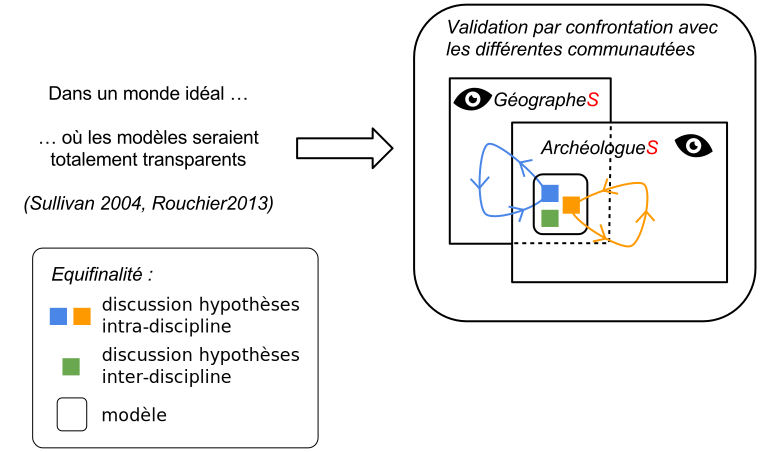
\includegraphics[width=1.1\linewidth]{vconfrontation.pdf}
  \end{sidecaption}
\end{figure}

Dans un \enquote{monde idéal} donc ou les modèles seraient totalement transparents (cad. sans erreurs, et dont la dynamique interne générale et propre à chaque hypothèses est complétement connue, voir figure \ref{fig:S_vconfrontation}) alors reste seulement en discussion les hypothèses, les implémentation d'hypothèses, et les critères d’évaluations choisis pour figurer au coeur du modèle. L’équifinalité impose donc qu’une partie de la validation (dont on sait qu’elle est contextuelle) opère dans cette confrontation avec les autres acteurs, et donc les autres point de vue de la communauté. 

Ainsi plus que les solutions techniques qui restent avant tout des moyens, c'est dans le processus de discussion et d'échange autour des hypothèses et des critères admis dans les modèles que notre connaissance sur les phénomènes réels est aussi amenée à progresser. Cette confrontation n'est pas statique, elle mobilise aussi une relecture des raisonnements ayant porté l'intégration des hypothèses ou des critères au modèle. %Ce n'est qu'à ce prix que des discussions à même de susciter la modification, l'hybridation et donc l'amélioration de ces mêmes modèles peuvent être mis en oeuvre. 

C'est exactement ce que nous dit \textcite{OSullivan2004}, il faut aller plus loin et donner toute les chances à cette discussion, en exposant le raisonnement, et les discours développés avec et autour des modèles : 

\foreignblockquote{english}[\cite{OSullivan2004}]{The process of model development, the possible outcomes it reveals and interpretations of those outcomes, taken together, constitute a geographical narrative, so that modellers become ‘makers’ of stories.}

Si on se place sur le plan de la reproductibilité, déjà assez peu mise en oeuvre cette dernières décennie \autocite{Wilensky2007a}, l'objectif porté par O'Sullivan nous impose d'aller encore plus loin en permettant aussi la reproduction des raisonnements autour de la construction des modèles. La variabilité exposé lors de la construction du modèle, les différents mécanismes, les différents critères, le jeu de leur mises en tension réciproque, tout cela devient partie intégrante d'une capsule temporelle autonome et reproductible qui peut être exporté, rejoué, modifié, discuté auprès des autres modélisateurs. De ce fait cette confrontation avec la propriété d'équifinalité des systèmes complexes passe d'une explicitation souhaité pour l'interdisciplinarité, à une explicitation plus que souhaitable, voire nécessaire pour la reconstruction et la discussion des raisonnements produits. Associé à la cumulativité et en donnant à voir autant ce qui marche, que ce qui ne marche pas dans nos modèles, on offre aussi cette possibilité d'une progression commune dans la déconstruction d'une partie de cette équifinalité. Comme le propose Denise Pumain, il s'agit de construire et de \enquote{défendre un projet unifié de quête d'intelligibilité} pour les sciences \autocite[157-158]{Mathieu2014}. 

Seulement jusqu'à présent l'évaluation des modèles n'est pas censé avoir de sens une fois sorti de son contexte de création, il y a donc un effort évident à faire pour se doter de l'ensemble des moyens nécessaire à l'exposition de ce contexte. La notion de \enquote{laboratoire virtuel} traditionnellement limité à l'expérimentation du modèle mute, et se pare aujourd'hui d'une acception légèrement différente. Des chercheurs \autocites{Schmitt2014, Amblard2003} ont voulu étendre cette notion pour y inclure également l'ensemble des méthodes et outils jugé nécessaire à l'étude de ce premier niveau d'expérimentation que représente la construction d'un modèle de simulation (la variation des hypothèses dans le modèle), désignant par ce fait un niveau supplémentaire d’expérimentation (la variation des outils et méthodes pour construire et étudier le modèle).  Il faut encore étendre et repenser l'analogie du \enquote{laboratoire virtuel}, faire de celui-ci une \enquote{place publique} et lui donner une profondeur temporelle afin de rejouer, en tout transparence, la construction des modèles au contact des données, des critères, des expérimentations \foreignquote{latin}{in vivo}.

